\section{Introduction}
During the last years the usage of smart-wearables (particularly smartwatches) has become more and more common with a number of 337 million units sold in 2019 and a forecast in sales of up to 527 million units by 2024 \cite{tenzer}.
With that also comes a natural demand in data protection caused by the amount of sensors built in these devices and their ability to capture sensible personal data (e.g. health informations).
Additionally smart devices can now also be used for many kinds of financial actions.
Since most wearables are connected to either the distributors or the respective mobile phones virtual assistant they should contain sensors for on one hand sound conduction and on the other hand audio recording.
In the current general smart-wearable design neither of these sensors is oriented towards the wearers arm.
With a change in position of these sensors smartwatches become eligible for functional biometric authentication.
Further motivation for this new authentication method comes from the fact that the previous classical methods (PIN, password...) are not suited for usage on smartwatches \cite{xu2017gait}.   
Nevertheless it is shown by Johnston \cite{johnston2015smartwatch} and Yang \cite{yang2015motionauth} in their respective works that there already are potential biometric authentication methods for smartwatches based on distinct hand or arm movements. 

From these preconditions a prototype is defined. This prototype uses a sound based functional biometric which gets applied to its wearers arm. 

\section{Related Work}
This section will give an overview on the terms of biometrics and its variations, authentication and also what defines an authentication system.
Additionally an insight into other works on biometric or smartwatch based authentication will be provided. 

\subsection{Authentication}
The term in general describes the process based on which a security systems tries to approve someone's claim of identity \cite{bhattacharyya2009biometric}.
Based on the input type of this claim the term authentication can be further subdivided into explicit and implicit authentication.
\textit{Explicit} authentication is more often also known as traditional authentication \cite{ranjan2016automatic}.
This includes providing knowledge like PIN or password, using a token but also performing gestures, fingerprints etc. from the biometrical field.

\textit{Implicit} authentication on the other hand describes mechanisms where a user does not provide a password, etc. directly.
Instead users are authenticated based on observations of their behavioural patterns\cite{jakobsson2009implicit}.
These observations are qualified for the use in e.g. biometrics since every individual has its own distinct habits which could be captured and analysed using different sensors \cite{shi2010implicit}.
Furthermore Shi, Jakobsson et al. state in their 2009 and 2010 works that implicit authentication is well suited for usage in combination with mobile smart-devices \cite{shi2010implicit} or portable computers \cite{jakobsson2009implicit}.
Based on this they propose three different application scenarios.
First as a second factor in combination with passwords, second as the main authenticator and thus replacing the usage of a password and last as additional assurance or an extra trust factor when performing e.g. financial actions on a mobile device.

\subsection{Biometrics}
\textit{Biometrics} (as in the Greek terms \textit{bios} and \textit{metrikos}) describes the utilization of an individuals physical traits or behaviour to clearly identify one from others. Contrary to the more known verification methods of PINs, passwords or ID-cards biometric identification does not rely on tokens or knowledge which could easily be forgotten or stolen, rather than unique personal traits like fingerprints, face geometry or the specific way someone interacts \cite[chpt. 1.1]{jain2007handbook}\cite{delac2004survey}.
Depending on the concept of usage a biometric system can be used in either verification or identification mode \cite[chpt. 1.3]{jain2007handbook}.
These two modes can also be differed by the use of \textit{positive} or \textit{negative identification} techniques \cite{wayman2005introduction}.

As already stated above biometric authentication uses an individuals personal traits as authentication tokens. Based on the kind of trait and the methods how they are provided the general term of biometrics can be further divided into behavioural and physiological biometrics.
Also a new kind of biometrics called functional biometrics was introduced by Liebers and Schneegass in 2020 \cite{schneegass2020functbiometric}.

\subsubsection{Behavioural Biometrics}
Behavioural biometrics refers to authentication systems in which the process of authentication is related to the behaviour of an individual \cite{bhattacharyya2009biometric}.
In most cases this process is conducted with the use of primarily gestures or other actions or movements capable of being performed in everyday life \cite{yampolskiy2008behavioural}.
Features which can be used for behavioural biometrics include e.g gait, keystrokes but also authentication patterns on smartphones could be used.
One main advantage compared to physiological biometrics is that some behavioural traits must not be collected actively but can be captured whilst performing any kind of different tasks \cite{yampolskiy2008behavioural}. 
Also there is no definite need for special hardware since the sensors needed are mostly built in smart wearables which are one of the main users of behavioural biometrics \cite{johnston2015smartwatch}.

\subsubsection{Physiological Biometrics}
Apart from behavioural biometrics the classification of physiological biometrics is also existent. 
This form of biometric authentication uses the more "static" traits of a users body as token such as e.g. fingerprints, hand geometry \cite{alsaadi2015physiological} or vein patterns \cite{faltaous2019vpid}.

A physiological system should also have a little higher accuracy than a behavioural one and it should be harder to use as an imposter since it is nearly impossible to identically copy a finger print, iris pattern, etc. \cite{koong2014user}, \cite{delac2004survey}.

\subsubsection{Functional Biometrics} With functional biometrics another novel kind of biometric authentication was introduced lately by Liebers and Schneegass \cite{schneegass2020functbiometric}.
This new concept stands as a major influence to this work notably with its first implementation in SkullConduct\cite{SkullConduct}. 
\begin{figure}
	\begin{center}
		\subfloat[Traditional Biometrics]{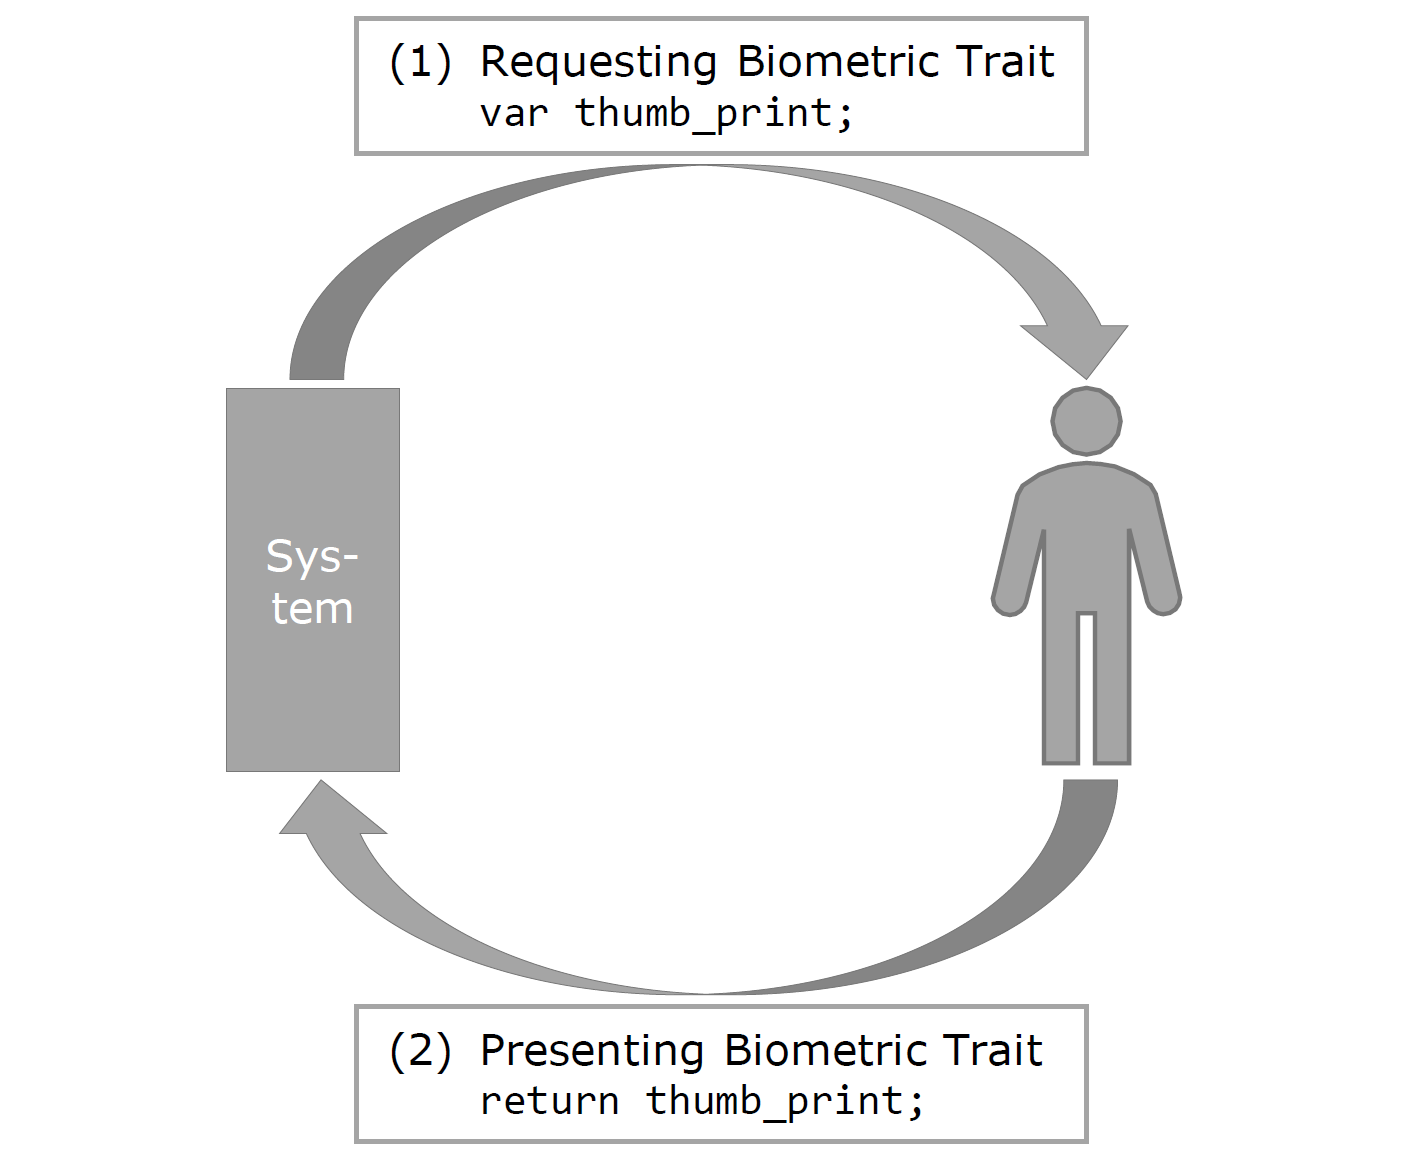
\includegraphics[width=0.4\textwidth]{Media/biometric_trad.png}\label{fig:tradBiom}}
		\hspace{0.5cm}
		\subfloat[Functional Biometrics]{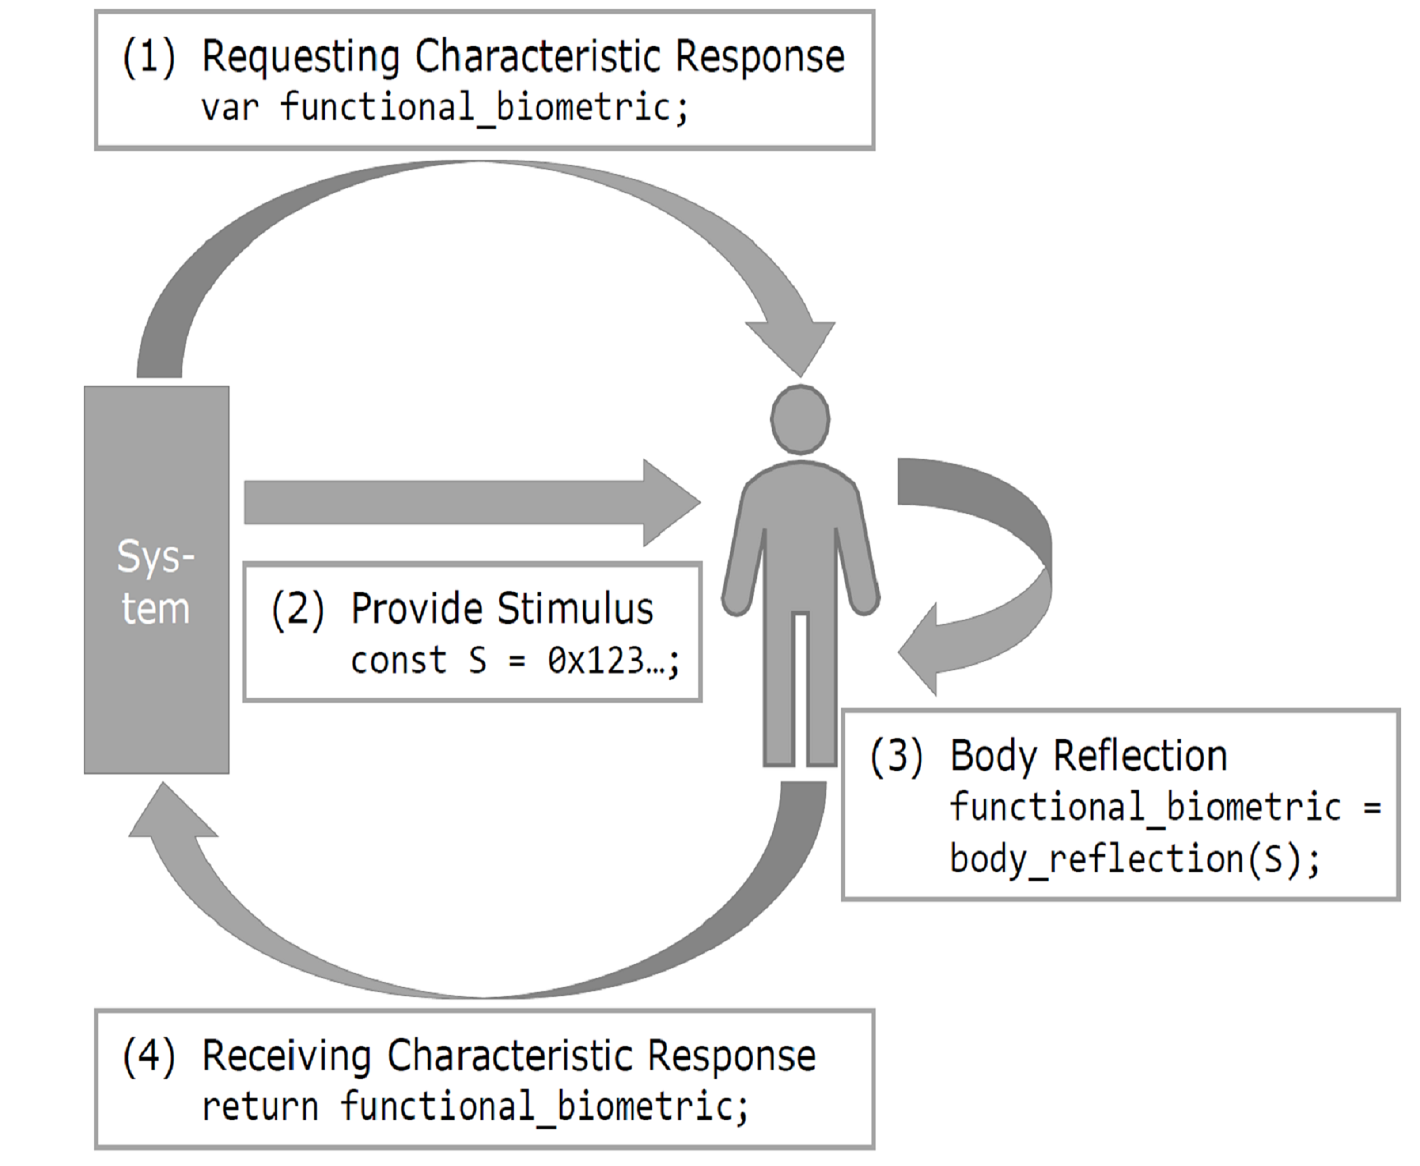
\includegraphics[width=0.4\textwidth]{Media/biometric_funct.png}\label{fig:functBiom}}
	\end{center}
	\caption{(a) shows the authentication process of a traditional biometric system where a characteristic response is created based on someone's unique trait.
	(b) shows the order of steps for functional biometrics when a stimulus is added to create the characteristic based on body reflections \cite{schneegass2020functbiometric}.}
	\label{fig:biometricsVersions}
\end{figure}

In this category of biometric authentication the authentication system provides an additional stimulus during the enrolment phase.
This stimulus is applied to the individuals body where it gets modified and afterwards captured (cf.~Figure~\ref{fig:functBiom}).
Due to different personal biological characteristics the modification of the stimulus is unique for each combination of user and stimulus.
Requirements Schneegass et al. proposed are two hardware components in form of a Stimulus Generation Unit (SGU) and a Body Reflection Sensor (BRS).
These two have to be designed as a dependence of the underlying biometric trait. Exemplarily when sound is used as the stimulus the SGU will be most likely some kind of microphone and the BRS a speaker.
During the enrolment process described above stimulus and its transformation are saved as a secret two-tuple ($x, f(x)$) with $ x $ being the stimulus and $ f(x) $ the transformation.
Now when the related user wants to authenticate the stimulus is reapplied and it is expected to get $f(x)$ as response again.
An additional security measure provided by functional biometrics is that when the stimulus gets leaked or lost the system is not fully compromised because the stimulus is only an exchangeable medium.
The secret stems from the body reflection function which is unique to the user, unknown and hard to manipulate.


As already mentioned before the SkullConduct work by Schneegass et al. is one of the key influences to this work. Not just because it is one of the first realizations for functional biometrics but it also 
serves as a source of inspiration for this work.
Schneegass et al. implemented a biometric authentication system using eyewear computers (e.g. Google Glass).
Therefore they used the concept of bone conduction which is already frequently used by hearing aids. SkullConduct, in this case, uses the bone conduction speaker of the Google Glass to emit a sound sample against the wearers head.
The sample which gets transformed due to the unique nature of each individuals head is captured by the glasses integrated microphone.
Results of this study  indicate that with all tested users SkullConduct had a probability of around 97\% when it comes just to identify a correct user.
Test of the system as an authentication tool showed an Equal Error Rate (EER) of around 6.9\% in average but with significant drops the shorter the used sample gets (less than 1 second).

Other work on authentication via smart devices includes e.g. the works from A. Johnston et al. who implemented a smartwatch based authentication module that used gait recognition \cite{johnston2015smartwatch}.
They adapted from previous work of theirs where gyro- and acceleration-sensors of smart phones were used to develop authentication methods \cite{kwapisz2010cell}.
The main thought behind the proposed use of gait authentication on smartwatches is that their place of wearing/usage is more consistent than the one of a smart phone and therefore more advantageous.
Each participants dataset includes both data from gyro- and acceleration-sensor.
Tests in regard of both design types showed that the general performance of authentication is way higher in average than the one of identification (e.g. 97.2\% compared to 79.2\%).
Additionally the overall performances of the acceleration-sensor was higher than the gyro-sensor.
Conclusions Johnston et al. drew from their results were that it is possible to authenticate someone sufficient enough using a smartwatch but they propose not to use the system for something other than a multi-modal biometric system at its current level. 
\newpage
%\section{Concept v1}
%The main motivation for this work lays in the concept of \textit{functional biometrics} \cite{schneegass2020functbiometric}.
%One already proposed implementation for this concept is the head mounted SkullConduct device \cite{SkullConduct}.
%There the HMD would emit a white noise sound sample against the wearers head whichs captured alteration is then used for the authentication.
%Limitations of SkullConduct are, amongst others, that it can only be applied on a fixed position whereas the concept provided here could be used on different body parts like arms or legs.
%This is relevant as it is more likely that the majority of people would use small smart devices rather than HMDs.
%
%Possible stimuli for the bracelet could be sound patters which use either white noise, frequency changes or little melodies.
%The stimulus can then be applied to the wearer on a regular base over the time the device is worn to ensure it is used by the correct user.
%Also if the stimulus used gets leaked or corrupted otherwise a functional biometric system does not need to be recalibrated completely.
%Since even the system itself does not really know the nature of the transformation function only a new stimulus and new sample data are needed.
%
%For the realisation of the described prototype a microcontroller will be used in combination with a microphone capsule and a little buzzer or speaker to capture and generate the stimuli described above.

\section{Concept}
With the introduction of functional biometrics space was created for the development of new mechanisms and variations in biometric authentication.
Contrary to other biometric systems which rely on e.g. fingerprints the body function used in functional biometrics can not be leaked or reproduced that easily.
This is due to the function being comprised of each individuals own body structure and bone density \cite{schneegass2020functbiometric}.

An already existing implementation approach to functional biometrics is the SkullConduct head mounted device (HMD) introduced by Schneegass et al. \cite{SkullConduct}.
There the HMD would emit a white noise sound sample against the wearers head.
The captured sound alteration is then used for the authentication.
Limitations of SkullConduct are, amongst others, that it can only be applied on a fixed position whereas the concept provided here could be used on different body parts like arms or legs.
This is relevant as it is more likely that the majority of possible users would prefer smaller smart devices such as smartwatches or other forms of bracelets, rather than HMDs on an everyday basis(cite?).
 
The authentication provided by the bracelet could be either used to secure data saved on the smart device or as multiple factor authentication for other connected devices like smartphones.

Possible stimuli for the bracelet could be sound patters which use either white noise, frequency changes or little melodies.
The stimulus can then be applied to the wearer on a regular basis over the time the device is worn to ensure it is used by the correct user.
Also if the stimulus used gets leaked or corrupted otherwise a functional biometric system does not need to be recalibrated completely.
Since even the system itself does not really know the nature of the transformation function only a new stimulus and new sample data are needed.

The realisation of this prototype consists of a microcontroller to generate the stimulus and process its transformation.
Additionally the controller is connected with a microphone capsule and a (piezo?-)speaker to emit and record the sound pattern.
 
\section{Implementation}
\subsection{Hardware}
The microcontroller used in this project is the LoRa 32 by Heltec Automation\footnote{\url{https://heltec.org/project/wifi-kit-32/}}.
The controller uses an 32bit dual-core microprocessor by espressif (esp32).
Other features include onboard Wi-Fi and Bluetooth as well as an 0.97 inch OLED display.
The controller can be powered using a micro-USB connection to a computer or an attachable lithium battery.

The implementation for the recordings is based around the use of an omnidirectional digital microphone\footnote{\href{https://www.amazon.de/Ambility-Omnidirektionales-Mikrofonmodul-I2S-Schnittstelle-Precision/dp/B07MW95PSS}{Ambility INMP441}}.
This microphone uses a digital I$^{2}$S-Interface to process its input. 
For the output of the generated stimuli a miniature speaker with a mylar-membrane\footnote{\href{https://www.conrad.de/de/p/lsf-15m-s-8-ohm-0-8w-miniatur-lautsprecher-geraeusch-entwicklung-85-db-0-500-w-1-st-710277.html}{LSF-15M/S}} is used which is able to conduct noise at up to 85 dB.

Further used hardware includes an SD-Card Reader equipped with an 32 Gigabyte SD-Card which is used as a cache to temporarily store the generated audiosamples.

\textit{\textbf{TODO: Komponentenverkabelung als Schematic oder Breadboardfoto}}
\subsection{Software}
\subsubsection{Development Environments}
The majority of code in this project was written in the Arduino IDE. 
This open-source IDE is designed and optimized for the use with microcontrollers from the arduino family.
It is also possible to add plugins for the support of other microcontroller chips like esp32 or the heltec LoRa family.
The IDE supports C and C++ as additional programming languages which can be processed by the microcontrollers.

Another major feature of the IDE is its ability to not only compile the designed sketches but also to flash them onto a microcontroller plugged into the computer via usb.
\pagebreak
\begin{figure}[H]
	\includegraphics[width=\linewidth]{Media/Controller_setup.png}
	\caption{The individual steps the microcontroller executes during its setup ordered as Statechart.}
	\label{fig:cntrlr_stp}
\end{figure}

\subsubsection{Code}
The code in this projects sketch is split up into three different parts - the main .ino-file and two additional .cpp files providing further code needed.

The main file locates the standard setup and loop functions for the microcontroller as well as the functionalities to generate the audio stimulus.
As seen in cf.~Figure~\ref{fig:cntrlr_stp} the setup functions main focus is initializing the different hardware components as well as starting the provided webinterface.

The webinterface can later on be used to apply the stimulus and record its alterations.
\textit{Also the webinterface can be used to download the generated audio sample from the SD Card attached to the microcontroller.}
To record the audio sample the i2s-interface is used.
Its exact specifications are defined in the i2s{\_}specs.cpp file. 

Information which is needed by the user can be printed onto the controllers OLED display.
For this purpose Heltec's version of the SSD1306 Library, which is included in the '\textit{heltec.h}' package, is needed.
To now print something onto the display it is necessary to call with
\begin{lstlisting}[style=inText]
	Heltec.display->drawString(int x, int y, String text)
\end{lstlisting}
x and y representing the coordinates on the display starting on the top-left from where the string is to be printed and text being the content to be printed. 

\paragraph{Stimulus Generation}
As for the stimulus' generation the used tone() function is implemented separately since the esp32 chipset does not support its functionalities naturally.
For this purpose the LED PWM functions can be used.
Using this functionality it is possible to control and alter both frequency and duty cycle of the output.

Initially these values are set within the \textit{ledcSetup()} function.
When changing the duty cycle at constant frequency it is possible to shift the pitch of the sound using the \textit{ledcWrite()} function.
When changing the frequency at constant duty cycle it is possible to generate different notes.
To do so the function \textit{ledcWriteTone()} has to be used instead of \textit{ledcWrite()}.
\begin{lstlisting}[frame=single, language={c++}, style=style,
				   caption={Function used to generate a single note using frequency and sound duration.}, label={lst:toneFunct},float=!htb]
void tone(int channel, int frequency_in_HZ,
		  		long durance_in_ms) {

	long delayAmount = (long)(1000000 / frequency_in_HZ);
	long loopTime = (long)((durance_in_ms*1000) / 
												 (delayAmount*2));

	for (int x = 0; x < loopTime; x++) {
		ledcWriteTone(channel, 3000);
		delayMicroseconds(delayAmount);
		ledcWriteTone(channel, 0);
		delayMicroseconds(delayAmount);
	}
	delay(20);
}
\end{lstlisting}

Based on these conditions the function tone() as seen in Listing~\ref{lst:toneFunct} uses the method ledcWriteTone() to generate sound\footnote{The function is taken from \href{https://gist.github.com/tagliati/1804108}{git} and altered slightly to work with the esp32 chipset}.
Additionally the parameters \textit{channel, frequency and durance} are required.
Using these parameters the function can determine the values for delay and loopTime representing pitch and sound duration respectively of the generated audio.
The third parameter is used to represent the PWM channel through which the sound will be forwarded.

Within the for-loop the ledcWriteTone() function is used to alternately set the PWM pin to high and low.
Between these alterations the pitch is set by setting a delay as previously computed.
As a final step a delay of 20 ms is set to separate the individual tone blocks from one another.

\paragraph{Recording the Sample}
über die i2s sachen...nochmal in youtube Video reingucken.

- Welche Params warum.

- Was tut i2s-init.

- was tut i2s-adc und warum bzw braucht man i2s-adc-data-scale.

- In Data-scale Wert mit 4096 /2048 etc...dient der Verstärkung, dabei je kleiner desto lauter

- irgendwas grafisches dazu?.

\paragraph{Webinterface}
Wie wird erstellt.

welche funktionen haben die einzelnen buttons.

Wie sieht interface in Browser aus!!! Screenshot von Firefox oder so.

Mit welchen Browsern funktioniert/getestet.

\section{Evaluation}
\section{Conclusion}
